\documentclass[convert]{standalone}
%\documentclass{article}

\usepackage{tikz}
\usetikzlibrary{bayesnet}

\begin{document}
    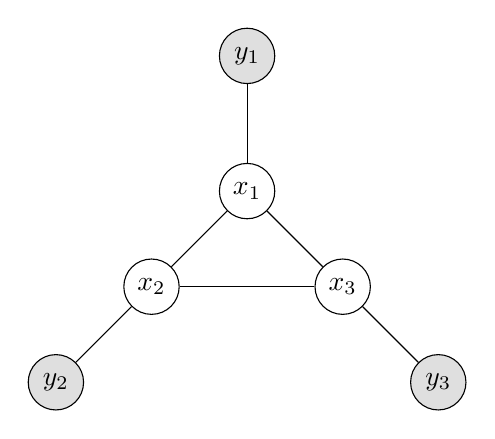
\begin{tikzpicture}
        
        % Nodes
    
        \node[latent] (x1) {$ x_{1} $};
        \node[latent, below left=of x1] (x2) {$ x_{2} $};
        \node[latent, below right=of x1] (x3) {$ x_{3} $};        
        \node[obs, above=of x1] (y1) {$ y_{1} $};
        \node[obs, below left=of x2] (y2) {$ y_{2} $};
        \node[obs, below right=of x3] (y3) {$ y_{3} $};
        
        % Edges
        
        \edge[-] {y1} {x1};
        \edge[-] {y2} {x2};
        \edge[-] {y3} {x3};
        \edge[-] {x1} {x2};
        \edge[-] {x1} {x3};
        \edge[-] {x2} {x3};

    \end{tikzpicture}
\end{document}